\chapter{Criação de Base de Dados}
\label{cap:banco}
Este capítulo tem como objetivo descrever a rede social Reddit e apresentar os
tópicos que foram selecionados para a análise de sentimentos. Após, é
demonstrada a ferramenta desenvolvida para a extração dos comentários destes tópicos e para a criação da base. Por fim, é
apresentada a validação da ferramenta desenvolvida.
\section{Rede Social Reddit}
\label{cap:Reddit}

O \textit{website} Reddit foi criado por Alexis Ohanian e Steve Huffman e teve
seu início em 2005 como um agregador de conteúdo e, atualmente, é o vigésimo terceiro \textit{website} mais acessado na
internet e o sétimo mais acessado nos Estados Unidos da América \cite{alexa}.
Os usuários do Reddit podem enviar \textit{links} com conteúdos externos
ao Reddit ou ainda mensagens de texto. A partir desse conteúdo, os seus
usuários podem votar para cima (\textit{upvote}) ou para baixo \textit{downvote},
influenciando na posição do conteúdo no \textit{website}. Além disso, seus
usuários podem enviar comentários como forma de expressar sua opinião (Figura \ref{fig:reddit}).


\begin{figure}[!htbp]
\centering

\includegraphics[height=300px]{imagens/reddit.png}
\caption{\textit{Website Reddit}:  As flechas demarcadas permitem efetuarmos
\textit{upvotes} ou \textit{downvotes}.}
\label{fig:reddit}
\end{figure}

O conteúdo do Reddit encontra-se distribuído em \textit{subreddits} que
funcionam como comunidades. Os usuários podem se inscrever nesses
\textit{subreddits}, recebendo as atualizações na sua página inicial, sendo
que dentre esses \textit{subreddits}, destacam-se:


\begin{itemize}
  \item \textit{/r/AskReddit}: esse \textit{subreddit} é utilizado para fazer
  perguntas gerais para outros usuários do Reddit. Esse \textit{subreddit}
  possui aproximadamente 16.941.540 inscritos.
  \item \textit{/r/worldnews}: esse \textit{subreddit} possui as notícias de
  todo o mundo, possuindo aproximadamente 16.570.600 inscritos.
  \item \textit{/r/IAmA}: IAmA é um estilização de \textit{'I am a'} ('Eu sou
  um'):
  a partir desse \textit{subreddit} os usuários podem fazer perguntas ao criador
  de um determinado tópico. Esse \textit{subreddit} possui aproximadamente
  16.990.160 inscritos.
\end{itemize}

% Dentre esses \textit{subreddits} podemos destacar alguns dos tópicos mais
% acessados no ano de 2016:
% 
% \begin{itemize}
%   \item \textit{/r/IAmA} - \textit{We're NASA scientists \& exoplanet experts.
%   Ask us anything about today's announcement of seven Earth-size planets
%   orbiting TRAPPIST-1!} - Tópico de perguntas e respostas com cientistas da
%   NASA após a descoberta dos planetas que orbitavam a estrela TRAPPIST-1.
%   \item \textit{/r/IAmA} - \textit{I’m Bill Gates, co-chair of the Bill \&
%   Melinda Gates Foundation. Ask Me Anything.} - Tópico de perguntas e respostas com Bill Gates.
%   \item \textit{/r/worldnews} - \textit{Fidel Castro is dead at 90.} - Link para
%   anúncio da morte de Fidel Castro.
%   \item \textit{/r/AskReddit} - \textit{[Serious]South Koreans of Reddit, how
%   did they teach you about the existence of North Korea in School when you were
%   young?serious replies only} - Tópico perguntando para os usuários sul coreanos
%   como que foi ensinado para eles sobre a existência da Coreia do Norte.
% \end{itemize}

% A identificação de padrões de sentimentos expressos por determinados grupos
% dessa comunidade, se faz útil visto que a partir dessa avaliação é possível construir
% ferramentas que apoiam decisões tanto de um ponto de vista político, como por
% exemplo, entender qual é a opinião sobre um determinado assunto de um conjunto
% de eleitores, tanto quanto um ponto de vista de negócios, para entender qual a
% opinião dos consumidores de um produto, ou de seu competidor, a respeito de um
% determinado assunto.

\section{Extração de Dados}
\label{cap:Extracao}

Para a extração de comentários do \textit{website} Reddit e para a criação da
base foi desenvolvido um \textit{crawler} ou robô de navegação. Esse robô foi
implementado na linguagem de programação Java e tem como objetivo a navegação
automática no conteúdo do \textit{website}, extraindo os dados e comentários referentes a um
determinado tópico. Após, os dados são armazenados em uma base de dados criada
em um banco de dados MySQL \cite{Widenius:2002:MRM:560480}.
Na Figura \ref{fig:crawler} tem-se a arquitetura do \textit{software}
desenvolvido. O código deste encontra-se no CD em anexo.

\begin{figure}[htbp]
\centering
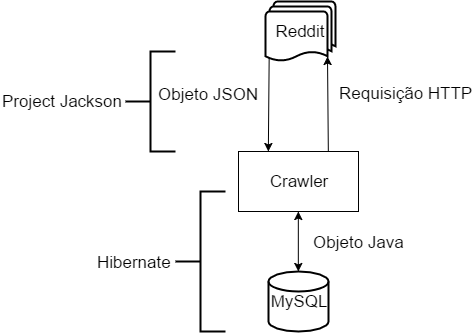
\includegraphics[height=225px]{imagens/arquitetura.png}
\caption{Arquitetura do \textit{Crawler}}
\label{fig:crawler}
\end{figure}

A partir do \textit{link} de um tópico, o robô efetua uma busca e a
extração dos dados relacionados a esse tópico. Para tanto, foi utilizada a
\ac{API} do Reddit, onde, inicialmente envia-se uma requisição utilizando o
sufixo ``.json'' (Por exemplo:
\textit{\url{https://www.reddit.com/r/iama.json}}) e, a partir dessa requisição,
o \textit{website} retorna um objeto \ac{JSON}. Uma vez que o \ac{JSON}
retornado possui 68 campos e que esses não se encontram
documentados, utilizou-se o \textit{website}
\textit{jsonschema2pojo}\footnote{http://www.jsonschema2pojo.org/ - O
\textit{website} jsonschema2pojo tem como objetivo a conversão de um esquema \ac{JSON} em
\textit{Plain Old Java Objects}\ac{POJO}, permitindo o \textit{download} da classe para a utilização.} para converter o
JSON retornado em um \textit{Plain Old Java Objects} (\ac{POJO}).

Após, foi utilizado o \textit{framework} Hibernate
\cite{Iverson:2004:HJD:1044870} para a criação do banco de dados e para a
persistência dos dados. O Hibernate é um \textit{framework} de
mapeamento objeto-relacional que tem como principal objetivo 
representar as tabelas de um banco de dados através de classes, ou seja, esse \textit{framework} tem como principal
característica a transformação das classes em Java em tabelas em um banco de
dados relacional.
No caso deste trabalho, ele é responsável pela criação das tabelas \textit{RedditPost} e
\textit{RedditThread}, relacionadas, respectivamente, com os comentários e o
tópico em questão. 

\section{Validação da Implementação}

Para validação da implementação desenvolvida foi selecionado o tópico:
\textit{``Canada will welcome you, Trudeau invites refugees as Trump bans
them''.}
A partir desse tópico, foram extraídos todos os comentários, sendo que
esses foram avaliados de forma manual. Após, esses comentários foram processados
utilizando-se a \ac{NLTK}, obtendo uma assertividade de 56\%.

Destaca-se que uma grande parte dos comentários que foram identificados de forma
incorreta, apresentavam a irônia como característica, como por exemplo, o
comentário \textit{``lol Good Luck Canada''}. A identificação da ironia através
da leitura textual é difícil até mesmo para um ser-humano, uma vez que o
texto pode não apresentar sinais de humor. De fato, a ironia para a análise de
sentimentos é considerado um tópico problemático sendo alvo de diversos estudos \cite{DBLP:conf/lrec/StranisciBFP16}.

Observou-se que nos demais comentários que foram identificados de forma
incorreta, o sentimento expresso não se encontrava no dicionário de
sentimentos padrão do \ac{VADER}. Desta forma, foi
utilizado o método de Propagação Dupla, que possui como principal objetivo
adicionar novas palavras ao dicionário
padrão do \ac{VADER} \cite{Qiu:2011:OWE:1970420.1970422}.

\section{Método de Propagação Dupla}

O método de Propagação Dupla, proposto por Qiu
\cite{Qiu:2011:OWE:1970420.1970422}, apresenta como objetivo resolver dois
problemas do \ac{NLP}, que são a expansão do dicionário e também a extração dos
alvos de um comentário. Os \textit{``Opinion targets"} ou alvos de opinião, são
palavras as quais sentimentos se referem. Por exemplo, na frase \textit{``Essa
música é muito boa''}, a palavra \textit{``boa''} demonstra o sentimento do
autor com relação a \textit{``música''}, tornando assim, a palavra
\textit{``música''} um alvo de opinião.

A extração dos alvos é interessante pois em uma mesma frase
podemos expressar opiniões sobre diferentes alvos. Além disso, podemos
ter opiniões diferentes sobre diferentes características de um alvo. Por
exemplo, na frase \textit{``Este celular é muito bom, porém a bateria dele é
péssima''}, tem-se que o produto em si é bom, porém, a opinião sobre a bateria
dele é negativa. De forma, a diminuir esses problemas, novas palavras e alvos
são adicionados ao dicionário padrão do \ac{VADER} partir da execução das quatro
tarefas que serão descritas na próxima seção.

\subsection{Adição de Palavras e Alvos ao Dicionário}

A \textbf{primeira tarefa}, é dividida em duas regras, sendo que a primeira
consiste na extração de alvos a partir de palavras que expressam um sentimento e
que já são conhecidas. Ou seja, são verificadas todas as palavras das quais a palavra que
expressa sentimentos depende. Caso essa palavra seja um substantivo, ela será
extraída e adicionada na lista de alvos. Por exemplo na frase \textit{``We have
a great president''} a palavra \textit{``great''} depende de \textit{``president''}, que é um substantivo. Neste caso, a palavra \textit{``president''} será adicionada na lista de alvos.

\[\textit{We have a } \underbrace{\textit{great president.}}_\text{president
\textrightarrow \text{ great}}\]

A segunda regra da primeira tarefa,
consiste em verificar se uma palavra que expressa um sentimento é dependente de
uma segunda palavra que depende de um substantivo.
Por exemplo, na frase \textit{``Trump is a great president.''} a palavra
\textit{``great''} depende da palavra \textit{``is''} que por sua vez depende da
palavra \textit{``president''} que é um substantivo. Neste caso, a palavra
\textit{``president''} será adicionada a lista de alvos.

\[\textit{Trump} \underbrace{\textit{is a great president.}}_\text{president
\textrightarrow \text{ is} \textrightarrow \text{ great}}\]

A \textbf{segunda tarefa} é a extração de novas palavras que expressam
sentimentos. Para isso, são utilizadas duas regras. Na primeira regra, é
verificada se a frase possui alguma palavra que se encontra na lista de alvos de
sentimentos, em caso positivo, é verificado se essa palavra possui algum dependente que seja um adjetivo. Por exemplo, na frase \textit{``Trump is a witty president.''}, a palavra \textit{``president''} foi
extraída na tarefa anterior, porém, a palavra \textit{``witty''} ainda não se
encontra no dicionário de sentimentos.
Desta forma, a palavra \textit{``witty''} será acrescida ao
dicionário de sentimentos uma vez que essa palavra é um adjetivo que não se
encontra no dicionário de sentimentos.


\[\textit{We have a } \underbrace{\textit{witty president.}}_\text{president
\textrightarrow \text{ witty}}\]

A segunda regra da tarefa dois
consiste em verificar se uma palavra alvo possui um dependente, que por sua vez
possui um adjetivo como dependente. Por exemplo, na frase
\textit{``Trump is a wholesome president.''} a palavra \textit{``wholesome''}, que é um
adjetivo, depende de \textit{``is''} que por sua vez depende de
\textit{``president''}. Neste caso, a palavra \textit{``wholesome''}
será adicionada ao dicionário de sentimentos uma vez que essa é um adjetivo que
ainda não existe no dicionário.

\[\textit{Trump} \underbrace{\textit{is a wholesome president.}}_\text{president
\textrightarrow \text{ is} \textrightarrow \text{ wholesome}}\]

A \textbf{terceira tarefa} consiste na extração de palavras alvo a partir de
palavras alvo que já se encontram na lista de alvos. A primeira regra desta
tarefa verifica se a frase possui alguma palavra na lista de alvos, e verifica se essa possui alguma
conjunção. Em caso positivo, a palavra após a conjunção é adicionada na lista
de alvos. Por exemplo, na frase \textit{``We have a great president and
leader."}, a palavra \textit{``president''} que foi extraída através
da primeira tarefa, possui a conjunção \textit{``and''} que a relaciona com a
palavra \textit{``leader''}, a qual não consta na lista de alvos. Neste
caso, a palavra \textit{``leader''} será adicionada a lista de alvos.


\[\textit{We have a great} \underbrace{\textit{president and
leader.}}_\text{president \textrightarrow \text{ and} \textrightarrow \text{
leader}}\]

A segunda regra da terceira tarefa verifica se dois substantivos
possuem uma palavra dependente em comum. No caso de um desses substantivos ser
uma palavra alvo, o outro também será adicionado na lista. Por exemplo, na frase
\textit{``Trump is a great president.''}, a palavra \textit{``president''} que
foi extraída através da primeira tarefa possui a palavra \textit{``is''} como
dependente, bem como a palavra \textit{``Trump''} também possui a palavra
\textit{``is''} como dependente. Desta forma, a palavra \textit{``Trump''} será adicionada a
lista de alvos.

\[\underbrace{\textit{Trump is a great president.}}_\text{Trump
\textrightarrow \text{ is} \textleftarrow \text{ president}}\]



A \textbf{quarta tarefa} tem como objetivo a extração de novos sentimentos a
partir de adjetivos já extraídos. A primeira regra desta tarefa, efetua a extração através
das conjunções presentes no texto. Por exemplo, para a frase \textit{``Trump is
witty and clever.''}, a palavra \textit{``witty''} possui uma conjunção
(\textit{``and''}), que a relaciona com a palavra \textit{``clever''}. Neste
caso, a palavra \textit{``clever''} será adicionada ao dicionário.

\[\textit{Trump} \underbrace{\textit{is witty and clever.}}_\text{witty
\textleftarrow \text{ and} \textrightarrow \text{ clever}}\]


A segunda regra da quarta tarefa, consiste em verificar-se dois adjetivos
dependem de uma mesma palavra. Se uma destas palavras pertence ao dicionário de
sentimentos, a outra também será adicionada ao dicionário. Por exemplo, na frase
\textit{``Trump is witty, clever''}, ambas as palavras \textit{``witty''} e
\textit{``clever''} dependem de \textit{``Trump''}. Neste caso, será extraída a
palavra \textit{``clever''} e adicionada ao dicionário.

\[\textit{Trump} \underbrace{\textit{is witty, clever.}}_\text{witty
\textleftarrow \text{ Trump} \textrightarrow \text{ clever}}\]

Por fim, é verificado se a lista de alvo ou o dicionário de sentimento sofreram
alterações, ou seja, se foram adicionadas novas palavras a essas listas. Em caso
positivo, as quatro tarefas serão executadas até que nenhuma palavra seja
adicionada nas listas.

\subsection{Atribuição de Pontuação às Novas Palavras}

Após a execução das quatro tarefas, se faz necessário definir a
pontuação relativa aos novos sentimentos e aos alvos que foram identificados
através do Método de Propagação Dupla. Essa atribuição é realizada da seguinte forma,
para as palavras que foram extraídas através da quarta tarefa, é utilizada a
mesma pontuação da palavra relacionada a essa nova palavra. Por exemplo, para a frase \textit{``Trump is
witty and clever.''}, a palavra \textit{``witty''} possui uma conjunção
\textit{``and''}, que a relaciona com a palavra \textit{``clever''}. Neste
caso, a palavra \textit{``clever''} terá a mesma pontuação da palavra
\textit{``witty''}.

Para a pontuação das palavras extraídas na tarefa dois, é realizado o seguinte
processo, na extração do alvo é atribuído a este alvo a mesma pontuação do
sentimento relacionado com ele. Por exemplo, na frase \textit{``We have a great
president''}, a palavra \textit{``president''} será adicionada a lista de alvos
de sentimentos com a mesma pontuação de \textit{``great''}, a qual está
relacionada. Após, essa pontuação é atribuída a palavra extraída a partir
da tarefa dois.
Por exemplo, no comentário \textit{``Trump is a wholesome president.''}, na
segunda tarefa, a palavra \textit{``wholesome''}, que foi extraída a partir da
palavra \textit{``president''}, irá receber a mesma pontuação da palavra
\textit{``great''}.

\subsection{Textos utilizados para o método de Propagação Dupla}
\label{sec:textos}

Para utilização do método de Propagação Dupla, é necessário utilizar-se de um
conjunto de textos para que sejam executadas as quatro tarefas. Segundo Qiu
\cite{Qiu:2011:OWE:1970420.1970422}, como as palavras podem ter diferentes
significados em diferentes contextos, é recomendado que este conjunto de textos pertença ao mesmo contexto que está sendo efetuada a análise de sentimentos. Por
exemplo, ao utilizar um conjunto de dados sobre notícias gerais, pode-se
determinar que a palavra \textit{``gucci''} é uma gíria similar a palavra
\textit{``good''}. Porém, o uso dessa palavra em comentários de roupas
apresenta um outro contexto, se referindo a uma marca de roupas.

A fim de se determinar o melhor conjunto de textos para utilização do método de
Propagação Dupla, foram utilizados dois conjuntos de dados de testes. No
primeiro conjunto de textos, considerou-se os comentários de todos os usuários
que comentaram o tópico \textit{``Canada will welcome you,” Trudeau invites
refugees as Trump bans them}. Mais especificamente, foram considerados os
últimos 1000 comentários destes usuários, totalizando 780063 comentários.

No segundo
conjunto de textos, foram considerados os comentários de usuários em tópicos
que apresentam o mesmo tema do tópico \textit{``Canada will welcome you,” Trudeau invites
refugees as Trump bans them}. Mais especificamente, foram utilizados os
seguintes tópicos:

\begin{itemize}
  \item
  \textit{Donald Trump to strip all funding from State Dept team promoting
  women's rights around the world - Leaked plan comes as First Daughter Ivanka
  defends her father's record with women}: esse tópico contém 9246
  comentários e encontra-se disponível em
  \textit{\url{https://www.reddit.com/r/worldnews/comments/67ivae/donald_trump_to_strip_all_funding_from_state_dept/}}.
  Esse tópico refere-se a decisão do presidente dos Estados Unidos da América,
  Donald Trump, em remover os fundos de promoção ao direito das mulheres.
  \item
  \textit{Sweden asks the U.S. to explain Trump comment on
  Sweden}: esse tópico contém 10927
  comentários e encontra-se disponível em
  \textit{\url{https://www.reddit.com/r/worldnews/comments/5uzetf/sweden_asks_the_us_to_explain_trump_comment_on/}}
  e se refere aos comentários feitos do presidente dos Estados Unidos da
  América, Donald Trump, sobre a Suécia.
  
  \item\textit{“Canada will welcome you,” Trudeau invites refugees as Trump bans
  them}: esse tópico contém 9113
  comentários e encontra-se disponível em
  \textit{\url{https://www.reddit.com/r/worldnews/comments/5qqa51/canada_will_welcome_you_trudeau_invites_refugees/}}
  e refere-se a declaração do primeiro ministro canadense sobre decisão de
  receber refugiados. Neste declaração, o primeiro ministro canadense afirma que
  os refugiados serão bem-vindos no Canadá.
\end{itemize}
 
Após a utilização do Método de Propagação Dupla utilizando esses dois conjuntos
de textos, foram obtidos os seguintes resultados para o tópico \textit{``Canada
will welcome you,” Trudeau invites refugees as Trump bans them}:
\begin{itemize}
  \item 58\% de assertividade na utilização do dicionário padrão.
  \item 59\% de assertividade na utilização do dicionário padrão com palavras
  extraídas a partir dos últimos 1000 comentários de todos os usuários que
  comentaram o tópico em questão.
  \item 62\% de assertividade na utilização do dicionário padrão com palavras
  extraídas a partir de comentários postados em tópicos relacionados ao mesmo
  tema.
\end{itemize}

Observa-se que os melhores resultados foram obtidos utilizando-se o método de
Propagação Dupla utilizando textos com assuntos relacionados. Desta forma, essa
será a abordagem utilizada no restante do trabalho.

\section{Restrição de Palavras Alvos}

Verificou-se que após a utilização do Método de Propagação Dupla, que os
comentários que não foram identificados de forma correta são comentários como: \textit{"...These laws are not "racist", morons keep hysterically throwing that word around and
its losing all meaning..."}, aonde que o sentimento expresso é negativo, porém,
a pessoa expressa um sentimento a favor da notícia em questão. 

Para amenizar esse problema, pode-se utilizar uma técnica que consiste em
restringir a análise à determinadas palavras alvos, ou seja, extrair somente os
sentimentos relacionados a uma determinada palavra alvo.
Por exemplo, no tópico \textit{````Canada will welcome you,'' Trudeau invites refugees as Trump bans them''}, é possível que a mesma pessoa expresse uma opinião positiva com relação
ao \textit{Canadá} e negativa com relação a \textit{Trudeau}. Ao se determinar
que desejamos analisar comentários sobre a palavra \textit{``Trudeau''},
pode-se definir \textit{Trudeau} como a palavra alvo para a análise,
sendo consideradas somente as frases relacionadas com essa palavra. Por exemplo, \textit{``Come enjoy our 15\%
tax :D edit: Trudeau is the most fake person ever. He always pulls this shit but
undercuts us Canadians all the time. He ain't getting voted in next
election.''}, será analisada somente a frase dependente da palavra
\textit{``Trudeau''}, que será \textit{``\ldots is the most fake person ever''},
evitando que a primeira frase \textit{``Come enjoy our 15\% tax :D\ldots''}, que
representa um sentimento positivo, afete a análise.

Restringindo a análise a palavra alvo \textit{``Trump''} para extração dos
comentários do tópico \textit{````Canada will welcome you,'' Trudeau invites refugees as Trump
bans them''}, foi obtida a assertividade de 65\%. A partir destes resultados,
optou-se pela utilização do método de \ac{VADER}, combinado com o método de Propagação Dupla e a
restrição de alvos para a execução dos testes que serão apresentados no Capítulo
\ref{cap:impl}.



